
%----------------------------------------------------------------------------------------
%	PACKAGES AND DOCUMENT CONFIGURATIONS
%----------------------------------------------------------------------------------------

\documentclass{article}

\usepackage[version=3]{mhchem} % Package for chemical equation typesetting
\usepackage{siunitx} % Provides the \SI{}{} and \si{} command for typesetting SI units
\usepackage{graphicx} % Required for the inclusion of images
\usepackage{natbib} % Required to change bibliography style to APA
\usepackage{amsmath} % Required for some math elements 
\usepackage{amssymb} % Required for other math elements 

\setlength\parindent{0pt} % Removes all indentation from paragraphs

\renewcommand{\labelenumi}{\alph{enumi}.} % Make numbering in the enumerate environment by letter rather than number (e.g. section 6)

%\usepackage{times} % Uncomment to use the Times New Roman font

%----------------------------------------------------------------------------------------
%	DOCUMENT INFORMATION
%----------------------------------------------------------------------------------------

\title{\texttt{Momentum and Energy Challenge Lab \\ Finding the Spring Constant \\ Physics 1 AP}} % Title

\author{\texttt{Michael Brodskiy}} % Author name

\date{\texttt{\today}} % Date for the report

\begin{document}

\maketitle % Insert the title, author and date

\texttt{
\begin{center}
\begin{tabular}{l r}
Date Performed: & 11.18.2019 \\
Partners: & Ryan Jacoby \\
& McKenna Dixon \\
& Graham Horrigan \\
Instructor: & Mrs. Halle
\end{tabular}
\end{center}}

% If you wish to include an abstract, uncomment the lines below
% \begin{abstract}
% Abstract text
% \end{abstract}

%----------------------------------------------------------------------------------------
%	SECTION 1
%----------------------------------------------------------------------------------------

\section{\texttt{Objective}}

\texttt{To find the spring constant, \textit{k}, of a cart, by designing our own lab with a limited amount of money}

% If you have more than one objective, uncomment the below:
%\begin{description}
%\item[First Objective] \hfill \\
%Objective 1 text
%\item[Second Objective] \hfill \\
%Objective 2 text
%\end{description}

\subsection{\texttt{Definitions}}
\label{definitions}
\begin{description}
\item[\textbf{Momentum}]
\texttt{Momentum, \textit{p} is equal to the mass, \textit{m}, times velocity, \textit{v}}.



\item[Potential Spring Energy]
\texttt{The Potential Spring Energy is equal to one half times the spring constant, \textit{k}, times the compression distance, \textit{x}, squared}


\item[Kinetic Energy]
\texttt{The Kinetic Energy is equal to one half times the mass, \textit{m}, times the velocity, \textit{v}, squared, or the antiderivative of momentum}

\item[Conservation of Momentum]
\texttt{Conservation of Momentum states that the Total Mechanical Energy, or all of the energies added together, is conserved. This means that we can set the kinetic energy equal to the potential spring energy, yielding:}



$$ \frac{1}{2} m  v^2  = \frac{1}{2} k x^2 $$


\end{description} 
 
%----------------------------------------------------------------------------------------
%	SECTION 2
%----------------------------------------------------------------------------------------

\section{\texttt{Experimental Data}}

\begin{center}
\begin{tabular}{lr}
\texttt{Mass of Cart with Flag} & \SI{276.4}{\gram}\\
\texttt{Mass of Cart with Flag and One Mass} & \SI{589}{\gram}\\
\texttt{Mass of Cart with Flag and Two Masses} & \SI{781.8}{\gram}\\
\texttt{Mass of Cart with Flag and Three Masses} & \SI{1033.7}{\gram}\\
\texttt{Mass of Cart with Flag and Four Masses} & \SI{1286.4}{\gram}\\
\texttt{Cart used} & \#7\\
\texttt{Balance Used} & \#2\\
\texttt{Spring Compression Distance $x$} & {51.61 mm}\\
\texttt{Flag Height} & {25mm} \\\\
\end{tabular}
\end{center}
%----------------------------------------------------------------------------------------
%	SECTION 3
%----------------------------------------------------------------------------------------

\section{\texttt{Purchases}}

\begin{center}
\begin{tabular}{lr}

\texttt{Photogate} & \$20\\
\texttt{iPad} & \$20\\
\texttt{Unlimited Balance Access} & \$10\\
\texttt{Flag} & \$5\\
\texttt{Calipers} & \$5\\
\texttt{Level} & \$3\\
\texttt{Four Masses} & \$5 each $-$ \$20\\
\texttt{Tape} & \$2\\\\
\hline
\texttt{Total} & \$85 \\\\
\end{tabular}
\end{center}

\texttt{With the purchases, a system was set up which looked as follows:\\\\\\}


\begin{figure}[h]
\begin{center}
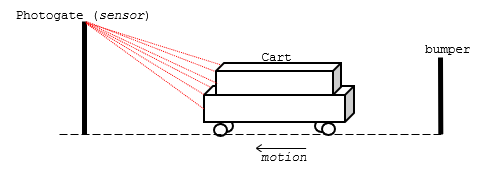
\includegraphics[width=\textwidth]{images/track.png} % Include the image placeholder.png
\textbf{\caption{\texttt{The Lab Setup}}}
\end{center}
\end{figure}

\texttt{The system can be used in tandem with the known variables, \textit{x}, \textit{m}, and \textit{v}, to solve for \textit{k} as follows:}

$$ \frac{1}{2} m  v^2  = \frac{1}{2} k x^2 \Longrightarrow mv^2 = kx^2 $$
$$ \therefore k = \frac{mv^2}{x^2}$$

\texttt{The velocity can be computed by using the photogate, the compression distance can be measured, and the mass can be weighed.}

%----------------------------------------------------------------------------------------
%	SECTION 4
%----------------------------------------------------------------------------------------

\section{\texttt{Collected Data}}

\begin{center}
\begin{tabular}{| l | c | c | c | c | c |}


\hline
 & \SI{276.4}{\gram} & \SI{589}{\gram} & \SI{781.8}{\gram} & \SI{1033.7}{\gram} & \SI{1286.4}{\gram}
\\ \hline
\texttt{Trial 1} & \SI{1.23}{\frac\meter\second} & \SI{.93}{\frac\meter\second} & \SI{.74}{\frac\meter\second} & \SI{.66}{\frac\meter\second} & \SI{.61}{\frac\meter\second}
\\ \hline
\texttt{Trial 2} & \SI{1.25}{\frac\meter\second} & \SI{.92}{\frac\meter\second} & \SI{.77}{\frac\meter\second} & \SI{.68}{\frac\meter\second} & \SI{.62}{\frac\meter\second}
\\ \hline
\texttt{Trial 3} & \SI{1.2}{\frac\meter\second} & \SI{.87}{\frac\meter\second} & \SI{.71}{\frac\meter\second} & \SI{.69}{\frac\meter\second} & \SI{.62}{\frac\meter\second}
\\ \hline
\texttt{Average} & \SI{1.2267}{\frac\meter\second} & \SI{.9067}{\frac\meter\second} & \SI{.74}{\frac\meter\second} & \SI{.6767}{\frac\meter\second} & \SI{.6167}{\frac\meter\second}
\\ \hline


\end{tabular}
\end{center}

%----------------------------------------------------------------------------------------
%	SECTION 5
%----------------------------------------------------------------------------------------

\section{\texttt{Graphing}}

\texttt{In order to produce a linear graph, the mathematical equation needs to be rearranged as follows:}
$$ \frac{1}{2} m v^2 = \frac{1}{2} k x^2 \Longrightarrow mv^2 = kx^2 \Longrightarrow v^2 = \frac{kx^2}{m}$$
$$ \therefore v = \sqrt{\frac{kx^2}{m}}$$

\texttt{To then obtain the slope, the variables must be separated into:}

$$ v = \sqrt{kx^2} \cdot \frac{1}{\sqrt{m}} $$

\texttt{The slope is given by $\sqrt{kx^2}$, which means the graph will be Average Velocity ($v$) plotted against Inverse Root Mass $\biggl(\frac{1}{\sqrt{m}}\biggr)$}

\begin{figure}
\begin{center}
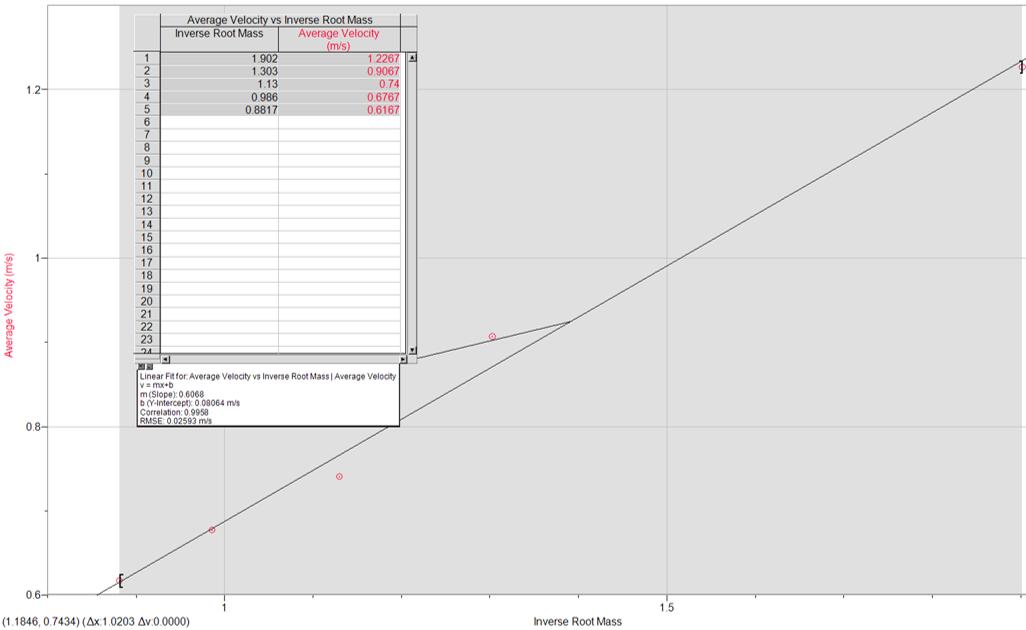
\includegraphics[width=145mm,height=105mm]{images/graph.png} % Include the image placeholder.png
\textbf{\caption{\texttt{Average Velocity vs Inverse Root Mass}}} 
\end{center}
\end{figure}

\begin{figure}
\begin{center}
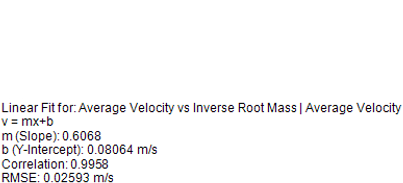
\includegraphics[width=80mm]{images/RMSE.png} % Include the image placeholder.png
\textbf{\caption{\texttt{Slope Specifications}}}
\end{center}
\end{figure}

%----------------------------------------------------------------------------------------
%	SECTION 6
%----------------------------------------------------------------------------------------

\newpage

\section{\texttt{Analysis \& Quality Control}}

\texttt{To find the spring constant, the line of best fit's slope must be set equal to the slope equation:}

$$ .6068 = \sqrt{kx^2} \Longrightarrow k = \frac{(.6068)^2}{(.05161)^2}$$
$$ \therefore k = 138.237 \frac{\text{N}}{\text{m}}$$

\texttt{This value can then be applied to find the initial velocity of a marble of mass \SI{65.36}{\gram}}

$$ 138.237 \cdot (.05161)^2 = .06536v^2 \Longrightarrow v = \sqrt{\frac{138.237 \cdot (.05161)^2}{.06536}} $$
$$ \therefore v = \SI{2.3735}{\frac\meter\second} $$

\texttt{This can then be applied to a kinetmatics equation to solve for the range:}

$$\Delta x = v_{ox}t + \frac{1}{2}a_{x}t^2$$\\

\texttt{The acceleration can be set to zero, because there is none in the horizontal direction, resulting in:}

$$\Delta x = v_{ox}t$$

\texttt{The time must be solved for using the vertical dimension:}

$$ v_{fy} = v_{oy} + a_yt \Longrightarrow 0 = v_{oy} + a_yt \Longrightarrow \frac{-v_{oy}}{a_y} = t$$

$$ \therefore t = \frac{-2.3735}{-9.80665} = \SI{.24203}{\second} $$

\texttt{By plugging in the time value, the range of the projectile is found to be:}

$$ \Delta x = (2.3735)(.24203) $$
$$ \Delta x = \SI{.574458}{\meter}$$


%-----------------------------------------------------------------------------------------
% SECTION 7
%-----------------------------------------------------------------------------------------

\section{\texttt{Error Analysis}}

\subsection{\texttt{Wear and Tear $-$ With every use, the spring becomes more worn, infinitesimally. This wear would cause the spring constant value to decrease, as the potential energy would be affected by the weakened spring.}}

\subsection{\texttt{Frictional Forces $-$ Throughout the experimentation there exist many frictional forces which are not accounted for. One such force is the force of friction exerted upon the wheels of the cart from the track. This would result in a lesser velocity value, and thus, a lower spring constant value. Another such force that would affect the launched ball is the frictional force from the air. This would cause the velocity to decrease at a faster rate, causing the range to be shorter than the calculated one.}}

\end{document}
